% Charlotte Geiger - Manuel Lippert - Leonard Schatt
% Physikalisches Praktikum

% Teilaufgabe X

\section{Teilaufgabe 1}

\begin{figure}[h]
    \begin{center}
        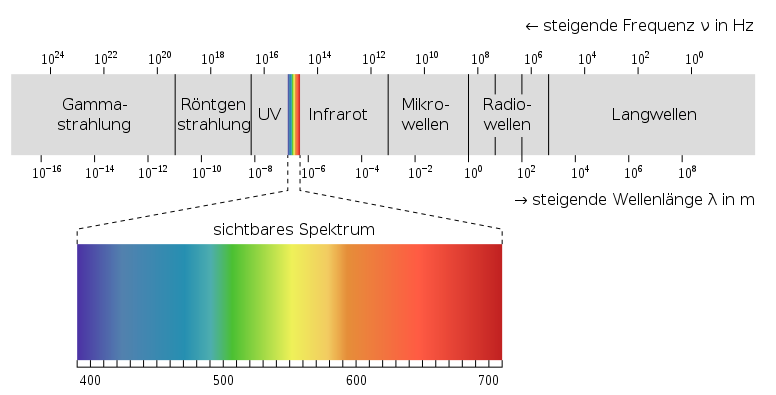
\includegraphics[width=12cm]{Bilder/emspekt.PNG}
    \end{center}
    \caption{Elekromagnetisches Spektrum}
    %\label{fig:meine-grafik}
   \end{figure}
\begin{itemize}
    \item Gammastrahlug: Gammastrahlug entsteht bei einem radioaktiven Gammazerfall. Man setzt sie
    im medizinischen Bereich ein, beispielsweise in der Strahlungstheraphie. Die hochenergetische Strahlung zerstört wucherndes Krebsgewebe indem es die entsprechende DNA zerstört. Sie
    kann nachgewiesen werden in einer Nebenkammer oder einem Geiger-Müller-Zählrohr.
    \item Röntgenstrahlung: Sie wird im medizinischen Bereich verwendet. Außerdem kann man es zur Untersuchung von Strukturen und zur Materialprüfung verwenden. Nachgewiesen kann die Strahlung 
    in Wechselwirkung mit Materie nachgewiesen werden. Man kann beispielsweise Fotoplatten einsetzen. Die Strahlung entsteht durch das Abbremsen von sehr schnellen Elektronen.
    \item UV: Die Strahlung kann sowohl natürlich als auch technisch entstehen. Lampen die UV-Strahlung erzeugen sind beipeilsweise Quecksilberdampf- und Quarzlampen. In diesen Lampen
    entsteht das Licht durch Anregung der jeweiligen Atomen in gasförmiger Phase durch Elektronen. Beim Zurückkehren in den Grundzustand emmittiern sie UV-Strahlung. Man kann die Strahlung
    detektieren, indem man den Photoeffekt nutzt. UV wird umfangreich in der Wirtschaft eingesetzt, unter anderem zur Materialprüfung oder zum aushärten von Polymeren.
    \item Sichtbares Spektrum: Der überwiegende Teil des auf der Erde vorkommenden Lichtes ensteht natürlichvorallem in der Sonne. Man kann es mit Fotoplatten detektieren.
    \item Infrarot: Es existieren Dioden, welche im Infrarotbereich abstrahlen. Man verwendet sie sehr oft bei Fernebedienungen. Infrar kann man mit thermischen Detektoren nachweisen.
    \item Mikrowellen: Mikrowellen entstehen in Laufzeitröhren oder Magnetrons. Die bekannteste technische Anwendung ist die Mikrowelle. Detektieren kann man sie mit einem Mikrowellenmessgerät.
    \item Radiowellen: Diese enstehen auf Radiosendemasten. Dort werden sie von Dipolenantennen erzeugt. Detektieren kann man sie mit einer passenden Antenne und einem Spannungsmessgerät.
    \item Langwellen: Auch diese können in der Natur vorkommen. Detektieren kann man sie mit einer passenden Antenne, hier vermutlich ein sehr langes Kabel und einem Spannungsmessgerät. 
\end{itemize} 